\documentclass[11pt,letterpaper]{article}
\usepackage{fullpage}
\usepackage{multicol}
\usepackage{amsmath}
\usepackage{amsfonts}
\usepackage{amssymb}
%\usepackage{pstricks, pst-node, pst-plot}

\ifx\pdfoutput\undefined
% we are running LaTeX, not pdflatex
\usepackage{graphicx}
\else
% we are running pdflatex, so convert .eps files to .pdf
\usepackage[pdftex]{graphicx}
\usepackage{epstopdf}
\fi

\newcommand{\ds}{\displaystyle}
\newcommand{\bv}{\mathbf}
\newcommand{\lv}{\langle}
\newcommand{\rv}{\rangle}

\begin{document}
\flushleft
\begin{multicols}{2}

\begin{large}\textbf{Math 116 Quiz 5: $\oint$ 11.1-11.6 (Differential Equations) \\
Tue 23 Oct 2012}\end{large}

\textbf{Name:  }\underline{\hspace{4pc}{\bf SOLUTIONS}\hspace{4pc}}

\vspace{.5in}

\end{multicols}

\pagestyle{empty}


\flushleft

You have 30 minutes to complete this quiz.  Eyes on your own paper and good luck!

\begin{enumerate}
\item  \textbf{Definitions/Concepts.} (1 pt ea) Consider a differential equation of the form
\[\frac{dH}{dt}=k(H-C),\]
where $k$ and $C$ are constants.
\begin{enumerate}
\item This is a \underline{\hspace{3ex}1st\hspace{4ex}} order differential equation.

\vspace{1pc}
\item What is the general solution to this equation?
\begin{align*}
\frac{dH}{dt} &=k(H-C) \\
\frac{dH}{H-C} &=kdt \\
\int\frac{dH}{H-C} &=\int kdt \\
\ln{|H-C|} &=kt+C' \text{ (note the constant $C'$ is not the same as the constant $C$)} \\
H-C &= e^{kt+C'} \\
&= Ae^{kt} \text{ (where $A=e^{C'}$ is a nonzero constant)} \\
H(t) &= Ae^{kt}+C
\end{align*}

\vspace{1pc}
\item What is the equilibrium solution to this equation?
\begin{align*}
H-C &= 0 \\
H &= C 
\end{align*}

\vspace{1pc}
\end{enumerate}
 
\item \textbf{Questions/Problems.} 

A box is dropped from an airplane.  The downward veleocity $v(t)$ of the box, once its parachute opens, satisfies the differential euqation
\[\frac{dv}{dt}=10-\frac{1}{10}(1+e^{-t})v^2.\]
\begin{enumerate}
\item (3 pts)
Suppose the parachute opens when the velocity of the box is 11 m/s.  Use Euler's method with three steps to approximate the velocity of the box one second after the parachute opens.
\[\begin{array}{|c|c|c|c|}
\hline
t & v(t) & dv/dt & \Delta v \\ [0.5ex]
\hline 
\hspace{4ex}0\hspace{4ex} & \hspace{3ex}11\hspace{3ex} & \hspace{3ex}-14.2\hspace{3ex} & \hspace{3ex}-7.1\hspace{3ex} \\ [0.5ex]
\hline
\hspace{4ex}0.5\hspace{4ex} & \hspace{3ex}3.9\hspace{3ex} & \hspace{3ex}7.556\hspace{3ex} & \hspace{3ex}3.778\hspace{3ex} \\ [0.5ex]
\hline 
\hspace{4ex}1\hspace{4ex} & \hspace{3ex}7.678\hspace{3ex} & \hspace{10ex} & \hspace{10ex} \\ [0.5ex]
\hline
\end{array}\]

What does your estimate say the velocity is after 1 second?

approximately $7.678$ m/s

\vspace{1pc}
%\hfill{\bf MORE QUIZ ON THE BACK --\textgreater}

\item (2 pts) Draw your Euler approximation on the following slope field:
\smallskip
\begin{center}
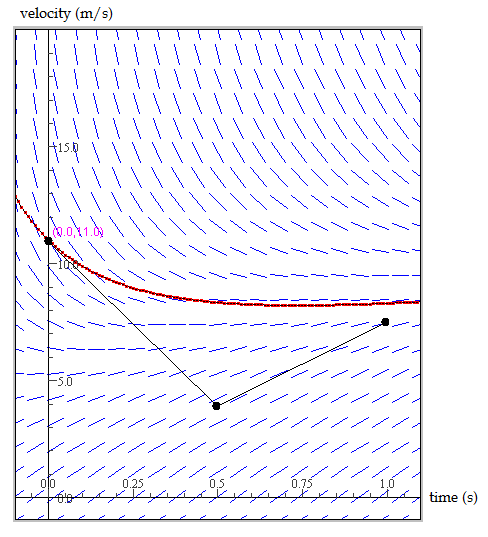
\includegraphics{quiz5solfld.png}
\end{center}

\item (2 pts) Say something {\bf about slope fields} to argue whether your approximation is an overestimate or an underestimate.

The approximation lies below the red solution curve, so it is an underestimate.

\vspace{1pc}
\end{enumerate}

\item \textbf{Computations/Algebra.} (1 pt ea) Find the solutions to the following differential equations subject to their given initial conditions.
\begin{enumerate}
\item $\frac{dy}{dx}+\frac{y}{3}=0,\;\;y(0)=10$
\begin{align*}
\frac{dy}{dx} &= -\frac{y}{3} \\
\frac{dy}{y} &= -\frac{dx}{3} \\
\ln{|y|} &= -\frac{1}{3}x+C \\
y &= ke^{-\frac{1}{3}x} \\
10 &= ke^{-\frac{1}{3}(0)};\quad k=-10 \\
y &= 10e^{-\frac{1}{3}x} \\
\end{align*}

\vspace{0.5pc}
\item $2\frac{du}{dt}=u^2,\;\;u(0)=1$
\begin{align*}
2\frac{du}{u^2} &= dt \\
-\frac{2}{u} &= t+C \\
-\frac{2}{t+C} &= u \\
1 &= -\frac{2}{0+C};\quad C=-2\;\;\text{ (switching sides in the equation then using the intial value)} \\
u &= -\frac{2}{t-2}
\end{align*}

\vspace{0.5pc}
\item $\frac{dz}{dy}=zy,\;\;z=1\text{ when }y=0$
\begin{align*}
\frac{dz}{z} &= y\,dy \\
\ln{|z|} &= \frac{y^2}{2}+C \\
z &= ke^{\frac{y^2}{2}} \\
1 &= ke^{\frac{0^2}{2}};\quad k=1 \\
z &= e^{\frac{y^2}{2}}
\end{align*}

\vspace{1pc}
\item $\frac{dz}{dt}=te^z,\;\;\text{ through the origin}$
\begin{align*}
e^{-z}dz &= t\,dt \\
-e^{-z} &= \frac{t^2}{2}+C \\
e^{-z} &= -\frac{t^2}{2}+C \text{ (constant is different now)} \\
-z &= \ln{\left|-\frac{t^2}{2}+C\right|} \\
z &= -\ln{\left|-\frac{t^2}{2}+C\right|} \\
0 &= -\ln{\left|-\frac{0^2}{2}+C\right|};\quad C=0 \\
z &= -\ln{\left|-\frac{t^2}{2}+1\right|}\;\;\text{ (assuming $|t|<\sqrt{2}$)} 
\end{align*}

\vspace{1pc}
\item $\frac{dw}{d\theta}=w+w\theta^2,\,\,w=5\text{ when }\theta=0$
\begin{align*}
\frac{dw}{w} &= (1+\theta^2)d\,\theta \\
\ln{|w|} &= \theta+\frac{\theta^3}{3}+C \\
w &= ke^{\theta+\frac{\theta^3}{3}} \\
5 &= ke^{0+\frac{0^3}{3}};\quad k=5 \\
w &= 5e^{\theta+\frac{\theta^3}{3}}
\end{align*}

\end{enumerate}

\end{enumerate}

\end{document}


